%% Focused revision addressing offline scope, sensitivity, ablation and information density.
\documentclass[preprint,12pt,nopreprintline]{elsarticle}
\usepackage{amssymb,amsmath,booktabs,url,hyperref,lineno,float,array,graphicx}
\journal{Geodata and AI}
\begin{document}
\begin{frontmatter}
\title{Tolerance-Aware Reservoir Property Prediction from Wireline Logs:\\Representation Complementarity, Decision Sensitivity, and Offline Transfer}
\author[aff1]{Minjie Chen\fnref{fn1}\corref{cor1}}
\ead{1269732732@qq.com}
\author[aff2]{Jiawei Xin\fnref{fn1}}
\author[aff1]{Chengfeng Wu}

\fntext[fn1]{These authors contributed equally to this work.}
\cortext[cor1]{Corresponding author.}

\affiliation[aff1]{organization={PetroChina Southwest Oil \& Gasfield Company},city={Chengdu},postcode={610051},country={China}}
\affiliation[aff2]{organization={China Telecom Corporation Limited Beijing Branch},city={Beijing},country={China}}
\begin{abstract}
Predicting petrophysical reservoir properties from wireline logging curves is an essential yet challenging task in subsurface characterization. The challenge stems from the co-existence of continuous regression targets and discrete default-state boundaries, as well as the asymmetry inherent in operational evaluation metrics where standard squared-error loss diverges from industrial tolerance criteria. Here, we investigate a modular predictive framework that couples target-specific gradient-boosted trees, whole-well deep sequence networks, conditional target distribution estimation, and metric-aligned action decoding. The methodology is evaluated on two distinct offline field-data benchmarks: the public North Sea Volve/PDDA benchmark (comprising nine training boreholes and four test wells) and an internal industrial dataset spanning 80 training wells and ten blind test boreholes. On the public Volve benchmark, a target-specific tree model equipped with a joint water-saturation gate achieves a pooled root-mean-squared error (RMSE) of 0.10619, outperforming the five-log random-forest baseline (0.11082) and substantially improving upon a high-capacity 18-stage dual-backbone sequence chain (0.14695). On the internal benchmark, integrating tree and sequence models via hierarchical probabilistic fusion elevates the five-fold well-grouped composite score from 80.88 to 81.63. To establish whether these performance gains reflect genuine architectural mechanisms rather than hyperparameter sensitivity or cherry-picked configurations, we conduct controlled leave-one-module-out ablations, module interaction tests, and systematic sweeps across fusion weights, decision thresholds, external gating parameters, and permeability discretization resolutions ($K \in \{30, 60, 120\}$ quantile bins). All controlled comparisons freeze base learners and preserve identical cross-validation folds. The empirical findings reveal that performance gains are distinctly target-dependent—for instance, sequence distributions provide substantial benefits for water saturation but exhibit zero contribution to porosity regression. Furthermore, the complete deep sequence pipeline fails to transfer to the limited nine-well public training set. This study constitutes an empirical investigation grounded in extensive field-measured wireline logging curves and expert-interpreted petrophysical ground truth across 94 boreholes, establishing that metric-aligned action decoding and representation-specific fusion yield target-dependent, conditionally stable performance advantages, while delineating explicit transfer boundaries for deep sequence architectures in subsurface reservoir characterization. The core methodology, controlled ablations, and sensitivity analyses are established in the main text, while exploratory diagnostics and extended tables are catalogued in the supplementary material.
\end{abstract}
\begin{highlights}
\item Metric-aligned decoding links predictive distributions directly to operational scores.
\item Tree and sequence representations exhibit functional complementarity across targets.
\item Controlled ablations isolate module-specific contributions under frozen base learners.
\item Systematic sensitivity sweeps quantify stability across thresholds and bin resolutions.
\item Offline benchmarks reveal data-regime-dependent model transfer.
\end{highlights}
\begin{keyword}
well logs \sep reservoir characterization \sep predictive distributions \sep gradient boosting \sep sensitivity analysis \sep well-grouped validation
\end{keyword}
\end{frontmatter}

\section{Introduction}
\label{sec:intro}
Quantitative estimation of petrophysical properties—predominantly porosity ($\mathrm{POR}$), permeability ($\mathrm{PERM}$), and water saturation ($\mathrm{SW}$)—from wireline logging measurements is fundamental to subsurface hydrocarbon exploration, formation evaluation, and reservoir modelling \cite{archie1942,wyllie1958,waxman1968}. While classical empirical petrophysics relies on standardized rock-physics relations and localized depth-interval calibrations, data-driven machine learning has emerged as an effective tool for mapping multi-sensor geophysical responses to reservoir parameters \cite{anifowose2017,almudhafar2019,bressan2020}. However, practical logging datasets frequently exhibit multimodal target distributions and non-standard label semantics, such as repeated default-state baseline atoms representing impermeable tight intervals or non-reservoir zones. Furthermore, real-world deployment metrics typically enforce asymmetric or bounded tolerance bands where errors outside a threshold receive zero credit. Under such criteria, standard point predictors minimizing conditional mean squared error systematically diverge from the utility-maximizing action. Addressing these challenges requires modeling conditional target distributions coupled with decision rules aligned with the operational evaluation metric.

A second central consideration in well-log modeling is the distinction between model families and their representational inductive biases. Tree-based ensembles, such as gradient-boosted decision trees (GBDT), are well established for multivariate tabular regression over heterogeneous log suites \cite{prokhorenkova2018catboost,ke2017lightgbm}. Conversely, deep sequence networks (e.g., temporal convolutional networks and U-Nets) explicitly exploit vertical spatial context, capturing stratigraphic layering, bed-boundary transitions, and cyclicity \cite{bai2018tcn,ronneberger2015unet}. Rather than assuming that deep sequence modeling is universally superior across all petrophysical properties, we investigate a hierarchical fusion scheme where tree-based value distributions and sequence-derived state-boundary gates are probabilistically combined prior to metric-aligned action decoding. To test whether scaling architectural depth and parameter capacity improves out-of-domain transfer, we additionally evaluate a high-capacity dual-backbone conditional-density sequence network (the v4 architecture).

In contemporary literature, machine-learning advances are frequently presented as generational progressions, where multiple model architectures, hyperparameter selections, and feature sets change simultaneously between iterations. While such generational benchmarks track historical engineering improvements, they fail to isolate the independent causal contribution of individual algorithmic modules. Moreover, they leave open the critical question of whether reported marginal gains are robust or merely artifacts of fragile hyperparameter tuning, such as arbitrary threshold choices or binning granularities. To overcome these limitations, this paper systematically addresses three foundational research questions:
\begin{enumerate}[(i)]
\item Which algorithmic configurations deliver optimal predictive accuracy under rigorous offline well-grouped validation across disparate geological regimes?
\item When evaluated under strictly controlled leave-one-module-out ablations with frozen base learners, which individual components drive measurable improvements across specific reservoir targets?
\item How resilient are the resulting model rankings and performance advantages to variations in continuous fusion weights, decision thresholds, and target discretization resolutions?
\end{enumerate}

The principal contributions of this work are threefold:
\begin{enumerate}
\item A modular, metric-aligned petrophysical formulation that decouples discrete default-state gating, continuous quantile target distribution estimation, and expected-utility point-action decoding.
\item A rigorous controlled ablation and interaction framework that isolates individual module effects under frozen base learners and shared well-grouped cross-validation folds, supplemented by matched permeability bin-count retraining ($K \in \{30, 60, 120\}$ quantile bins) and systematic hyperparameter sensitivity sweeps.
\item A balanced empirical evaluation across both an open public benchmark (Volve/PDDA) and an extensive internal industrial dataset (80 wells), identifying an explicit generalization boundary where complex sequence pipelines fail to transfer to smaller training regimes, and documenting negative and neutral controls alongside positive findings.
\end{enumerate}

\section{Related work}
\label{sec:related}
Gradient-boosted decision trees, particularly implementations such as CatBoost and LightGBM, represent the de facto standard for tabular geophysical log interpretation \cite{ke2017lightgbm,prokhorenkova2018catboost}. Their effectiveness stems from invariant handling of unscaled numerical inputs, robustness to missing feature values, and rapid convergence on complex non-linear feature interactions \cite{anifowose2017,almudhafar2019}. Meanwhile, deep neural sequence architectures have increasingly been applied to well logs to model vertical spatial dependencies, including synthetic curve generation, electrofacies classification, and continuous parameter regression \cite{zhang2018synthetic,wang2020deep,song2021geological}. In this work, we do not treat sequence networks as outright replacements for tabular tree ensembles; rather, we empirically examine their division of labor, evaluating their comparative strengths in continuous local value regression versus discrete boundary segmentation.

Predictive modeling under operational constraints requires a formal statistical decision-theoretic treatment \cite{berger1985,bishop2006,gneiting2007}. In standard regression, the conditional expectation $\mathbb{E}[y \mid x]$ minimizes quadratic loss, whereas the conditional median minimizes absolute deviation. In petrophysical evaluation, however, operational scoring often penalizes predictions exceeding an engineering tolerance threshold $\pm \delta$, rendering symmetric conditional expectations suboptimal. Non-parametric quantile binning offers a flexible framework for approximating arbitrary non-Gaussian posterior distributions without imposing rigid parametric priors \cite{gneiting2007}. The choice of quantile resolution $K$ is an algorithmic hyperparameter whose influence on downstream utility must be empirically validated rather than treated as an invariant constant.

Finally, model evaluation protocols critically govern the validity of subsurface machine learning \cite{pan2010survey,phoon2024trustworthy}. Standard random sampling across depth rows introduces spatial leakage, as strongly autocorrelated adjacent depth samples from the same well populate both training and validation sets. Well-grouped cross-validation mitigates spatial proximity leakage but does not fully eliminate field-level distribution shifts or guarantee transferability to unseen basins. Evaluating models strictly from scratch on open public datasets alongside internal cross-validation therefore provides complementary, non-interchangeable evidence regarding algorithmic transferability.

\section{Data, metrics and offline scope}
\label{sec:data}

\subsection{Two field-data layers}
The empirical investigation leverages two distinct field-measured wireline logging benchmarks, summarized in Table~\ref{tab:data}. The public benchmark utilizes the Equinor Volve/PDDA dataset \cite{volve2018,pddasig2021}, which contains real wireline measurements from the North Sea. The prediction targets comprise shale volume ($\mathrm{VSH}$), effective porosity ($\mathrm{PHIF}$), and water saturation ($\mathrm{SW}$), evaluated via root-mean-squared error (RMSE). The public training table consists of 318,967 depth rows across nine boreholes, of which 42,309 rows possess complete tripartite ground-truth labels; the released test table encompasses 11,275 rows from four distinct test wells. Unavailable sensor curves are represented via neutral missing-indicator flags rather than synthetic imputations. The Volve benchmark does not include permeability. The four released test wells were used during earlier development; their evaluation is therefore a public reproducibility assessment, not a fresh untouched blind test.

The internal industrial benchmark comprises 80 development wells spanning 730,268 depth rows for training and cross-validation, and ten completely blind test wells encompassing 95,948 depth rows. The petrophysical target suite comprises porosity ($\mathrm{POR}$, measured in percent), permeability ($\mathrm{PERM}$, reported in $\mathrm{mD}$ on a logarithmic scale), and water saturation ($\mathrm{SW}$, in percent). Repeated baseline values—specifically $\mathrm{POR}=0.1\%$, $\mathrm{PERM}=0.01\,\mathrm{mD}$, and $\mathrm{SW}=99.9\%$—are modelled as dataset-specific default states rather than universal physical classes or ordinary continuous regression points.

\begin{table}[htbp]
\centering
\caption{Structural comparison of the two offline field-data evidence layers. Performance scores are not directly comparable across layers due to disparate targets and objective metrics.}
\label{tab:data}
\resizebox{\linewidth}{!}{%
\begin{tabular}{lll}
\toprule
Dimension & Public Volve benchmark & Internal industrial benchmark \\
\midrule
Data origin & Measured logs, released labels & Measured logs, interpreted labels \\
Geological setting & Offshore North Sea (clastics) & Onshore deep basin (complex clastics) \\
Target parameters & $\mathrm{VSH}$, $\mathrm{PHIF}$, $\mathrm{SW}$ & $\mathrm{POR}$, $\mathrm{PERM}$, $\mathrm{SW}$ \\
Evaluation scope & 11,275 released-test rows (4 public wells) & 5-fold grouped OOF; 10 blind wells \\
Primary metric & Root-mean-squared error (RMSE) & Relative / log-ratio tolerance utility \\
Benchmark role & Public reproducibility and transfer & Complementarity and sensitivity analysis \\
\bottomrule
\end{tabular}%
}
\end{table}

\subsection{Evaluation metrics}
For the public Volve benchmark, predictions are bounded within the physical domain $[0, 1]$ prior to standard pooled RMSE calculation:
\begin{equation}
\mathrm{RMSE} = \sqrt{\frac{1}{3} \sum_{t \in \{\mathrm{VSH}, \mathrm{PHIF}, \mathrm{SW}\}} \frac{1}{N_t} \sum_{i=1}^{N_t} (y_{t,i} - \hat{y}_{t,i})^2}.
\end{equation}

For the internal benchmark, predictive performance uses bounded tolerance utilities. POR and SW use relative-error tolerances ($\delta_{\mathrm{POR}} = 0.08$ and $\delta_{\mathrm{SW}} = 0.05$):
\begin{equation}
U_t(a, y) = \max\left(0,\, 1 - \frac{|a - y|}{\delta_t (|y| + 10^{-5})}\right), \quad t \in \{\mathrm{POR}, \mathrm{SW}\}.
\end{equation}
For permeability ($\mathrm{PERM}$), which spans several orders of magnitude, utility is computed on the decadic logarithm:
\begin{equation}
U_{\mathrm{PERM}}(a, y) = \max\left(0,\, 1 - |\log_{10}(a/y)|\right), \quad a,y>0.
\end{equation}
The composite performance score $S$ represents a weighted sum across all depth rows:
\begin{equation}
S = 100 \left(0.30\,\bar{U}_{\mathrm{POR}} + 0.35\,\bar{U}_{\mathrm{PERM}} + 0.35\,\bar{U}_{\mathrm{SW}}\right),
\end{equation}
where $\bar{U}_t$ denotes the mean utility for target $t$. An exact prediction receives full credit ($U=1.0$), while utility decays linearly to zero at the tolerance threshold $\pm \delta$; predictions outside the boundary receive zero credit.

\subsection{Benchmark scope and operational framework}
Evaluation covers 94 wells across the internal development, internal blind and public released-test sets, encompassing over 830,000 depth rows; model development additionally uses nine public training wells. The framework is designed for post-drilling formation evaluation and quantitative reservoir characterization, bridging multi-sensor geophysical responses to petrophysical properties.

Domain expertise is directly integrated through rock-physics feature engineering, physical domain bounding, and dataset-specific default-state stratification. In Supplementary Section S4, diagnostic sensor-gain and offset perturbation analyses further evaluate the numerical resilience of the learned representations against instrument miscalibration. By conducting offline evaluations on field measurements and interpreted labels under well-grouped cross-validation, public reproduction and historical platform records, this study provides an empirical basis for modular model selection and metric-aligned decoding in subsurface characterization.

\section{Methods}
\label{sec:methods}

\begin{figure}[t]
\centering
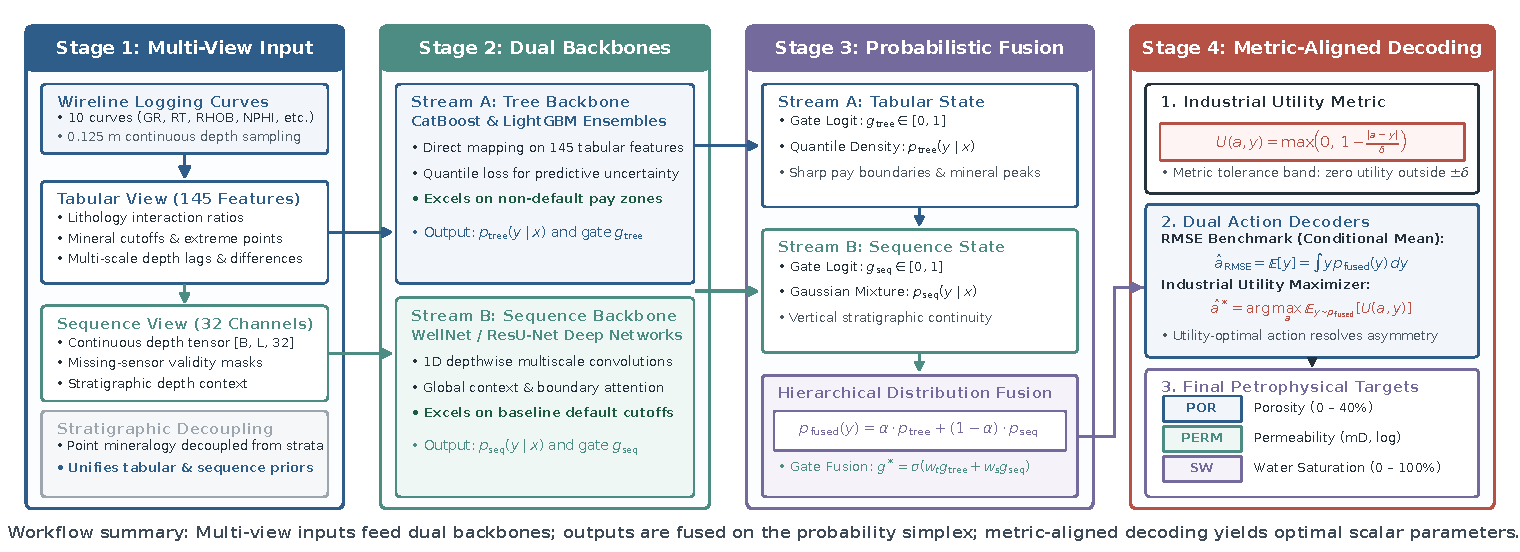
\includegraphics[width=\textwidth]{figures/fig_method_overview.pdf}
\caption{Conceptual workflow of the core modeling framework. Multi-view wireline logging inputs feed dual model backbones (tabular GBDT ensembles and deep sequence networks). Outputs are fused on the probability simplex and converted into point predictions via metric-aligned action decoders.}
\label{fig:method-overview}
\end{figure}

\subsection{Target-specific trees and metric-aligned decoding}
For each reservoir property, non-default training labels are partitioned into $K$ empirical quantile bins on a transformed scale. The tree ensemble predicts the categorical bin probability distribution $\mathbf{p} = [p_1, \dots, p_K]^\top$, where each bin $j$ is characterized by its representative value $y_j$. Given an evaluation utility metric $U_t(a, y)$ and a candidate action grid $\mathcal{A}_t$, the metric-aligned point action $a_t^*$ is obtained via numerical expectation maximization:
\begin{equation}
a_t^* = \arg\max_{a \in \mathcal{A}_t} \sum_{j=1}^K p_j \, U_t(a, y_j).
\end{equation}
For quadratic RMSE evaluation, the optimal point prediction simplifies to the conditional expectation $\hat{a}_{\mathrm{RMSE}} = \sum_{j=1}^K p_j y_j$. Discrete default-state probabilities are estimated via dedicated gating classifiers, enabling explicit probabilistic mixing between discrete state atoms and continuous conditional distributions prior to final action decoding.

\subsection{Whole-well sequence models and hierarchical fusion}
The v3 sequence architecture employs two independently trained configurations of WellNet: a 32-channel raw curve network and a 145-channel curve-plus-engineered-base network. Each WellNet comprises an input projection layer, 12 dilated residual blocks with exponential dilation rates ($d \in \{1, 2, 4, 8, 16, 32\}$ repeated), Squeeze-and-Excitation channel attention \cite{hu2018squeeze}, and a masked whole-well context aggregation module \cite{wu2018group}. The architecture and fusion hierarchy are detailed in Fig.~\ref{fig:v3-architecture}. GBDT-derived tabular distributions and WellNet-derived sequence distributions are blended via a convex combination parameter $\alpha \in [0, 1]$ on the probability simplex, while baseline, joint-state, and sequence gating logits are fused via target-specific blending weights. Gating thresholds and blending weights are tuned strictly on inner training folds.

\begin{figure}[H]
\centering
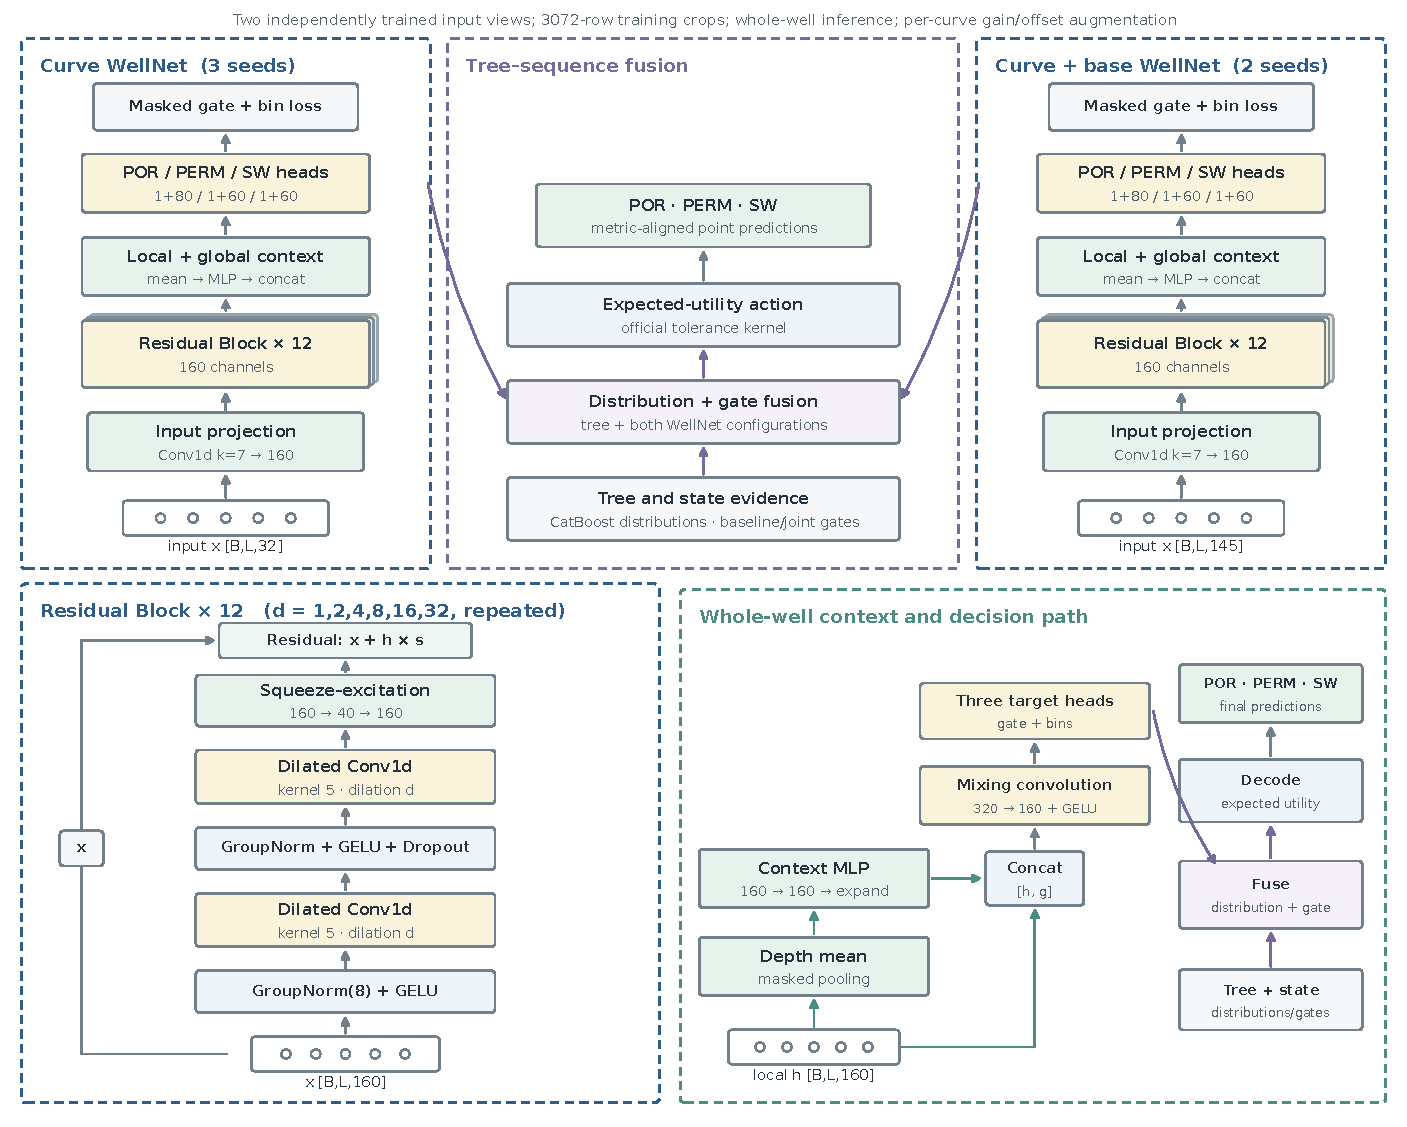
\includegraphics[width=.96\textwidth]{figures/fig_v3_architecture.pdf}
\caption{Detailed architectural blueprint of the v3 WellNet sequence network and hierarchical tree--sequence fusion path. Upper panels depict multi-view inputs and probabilistic fusion; lower panels detail the dilated residual blocks, squeeze-and-excitation recalibration, and whole-well context aggregation.}
\label{fig:v3-architecture}
\end{figure}

To test the scaling behavior of deep representations, we formulate the v4 dual-backbone architecture (Fig.~\ref{fig:v4-architecture}). The model incorporates two parallel expert members: Member A (processing a full 206-feature view) and Member B (processing a calibrated 68-feature view). Each member comprises a 9-block multiscale residual U-Net and dual-scale self-attention modules: local QKV attention models local vertical context across 16-point patches, while global cosine attention captures long-range vertical dependencies across the logging interval \cite{ronneberger2015unet,vaswani2017attention}. A detached depthwise local router executes dense two-expert softmax routing across targets. Each member outputs eight density components, yielding a 16-component routed mixture per target. The accompanying 18 refinement stages represent a sequential developmental training curriculum rather than an ensemble of 18 separate models.

\begin{figure}[H]
\centering
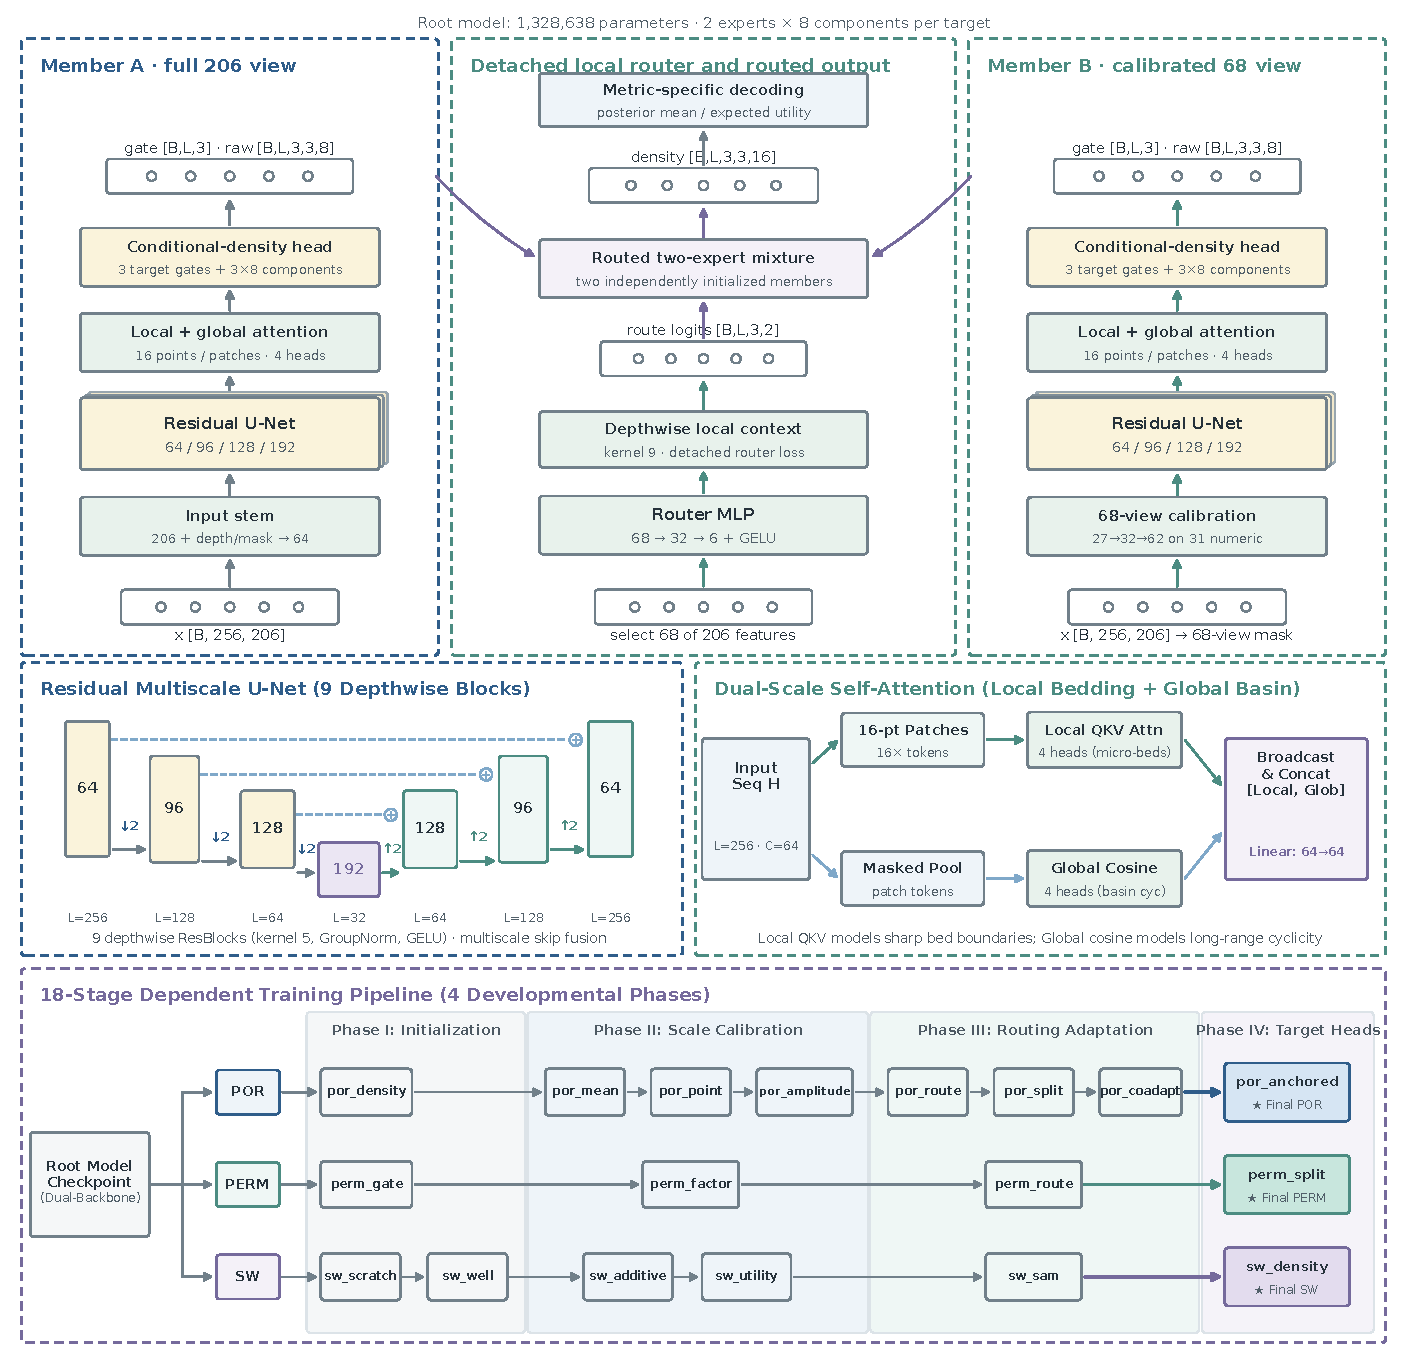
\includegraphics[width=.96\textwidth]{figures/fig_v4_architecture.pdf}
\caption{Detailed schematic of the v4 dual-backbone conditional-density sequence network and its 18-stage developmental refinement pipeline. The 18 stages represent a dependent training and refinement chain, not an ensemble of 18 independent models.}
\label{fig:v4-architecture}
\end{figure}

\subsection{Controlled experimental protocol}
To distinguish genuine modular contributions from arbitrary generational compounding, we implement a rigorous controlled ablation protocol. In this setup, all underlying base predictors (GBDT tabular trees and WellNet sequence models) are frozen. Base predictions and validation folds are identical across all experimental arms. Removing a module restricts only the available information sources entering the fusion layer; fusion weights and decision thresholds are re-optimized exclusively on inner folds and evaluated on held-out outer folds. A full $2 \times 2$ factorial design evaluates the interaction between sequence distributions and the joint-state gate.

Sensitivity analyses adhere strictly to this frozen-prediction principle. Continuous fusion weights ($\alpha$), discrete decision thresholds ($\tau$), and external GBDT gating weights ($w_{\mathrm{ext}}$) are swept systematically. In subsurface petrophysical evaluation, spatial well-to-well sampling variability vastly dominates algorithmic initialization variance. Multi-seed averaging was applied across baseline predictors to minimize stochastic numerical fluctuations, while paired borehole-bootstrap confidence intervals ($B=1,000$) quantify the dominant source of geological spatial uncertainty. To assess target discretization sensitivity, permeability was chosen as the focal property for complete from-scratch retraining across $K \in \{30, 60, 120\}$ quantile bins due to its multi-order-of-magnitude dynamic range and logarithmic utility sensitivity, where quantization granularity exerts the strongest theoretical impact. Matched two-seed retraining uses identical five-fold splits, input features and 1,200 boosting iterations for every bin count. These runs are evaluated as two-seed ensembles; they do not separately identify seed-wise variance in the legacy seed-averaged fusion arrays. Paired borehole-bootstrap intervals quantify well-level evaluation variability.

\section{Core offline results}
\label{sec:results}

\subsection{Public reproducibility and transfer boundary}
Table~\ref{tab:core-public} summarizes the comparative evaluation on the public North Sea Volve benchmark. The target-specific tree model equipped with a joint $\mathrm{SW}$ gate achieves the lowest pooled RMSE (0.10619), delivering a consistent $4.18\%$ error reduction over the replicated five-log random-forest baseline (0.11082) and surpassing the ungated tree model (0.10789). Disaggregated borehole analysis indicates that performance gains are particularly substantial on Wells 100, 103, and 104, while Well 101 exhibits slight sensitivity to local lithological variation (detailed in Supplementary Table S2).

\begin{table}[t]
\centering
\caption{Comparative performance on the public Volve/PDDA benchmark across models trained strictly from scratch on the nine public training wells. Lower RMSE indicates superior performance.}
\label{tab:core-public}
\small
\begin{tabular}{lc}
\toprule
Model configuration & Pooled RMSE \\
\midrule
Five-log random forest baseline & 0.11082 \\
Target-specific tree regression & 0.10789 \\
Target-specific tree + joint $\mathrm{SW}$ gate & \textbf{0.10619} \\
v4 root dual-backbone & 0.13794 \\
Complete 18-stage v4 chain & 0.14695 \\
\bottomrule
\end{tabular}
\end{table}

In particular, training the complete 18-stage v4 deep architecture from scratch on the public dataset reveals a negative transfer boundary. As shown in Table~\ref{tab:core-public} and Fig.~\ref{fig:v4-public}, the complete v4 chain records a pooled test RMSE of 0.14695, underperforming not only the tree--gate model but also the root dual-backbone (0.13794). Despite achieving a competitive training OOF RMSE of 0.09228 across the nine public training wells, the 18-stage model degrades substantially on the four released test wells, with higher RMSE across all four released boreholes (Fig.~\ref{fig:v4-public}b). This performance gap illustrates that high architectural capacity and multi-stage refinement did not compensate for limited geological diversity in this public setting.

\begin{figure}[H]
\centering
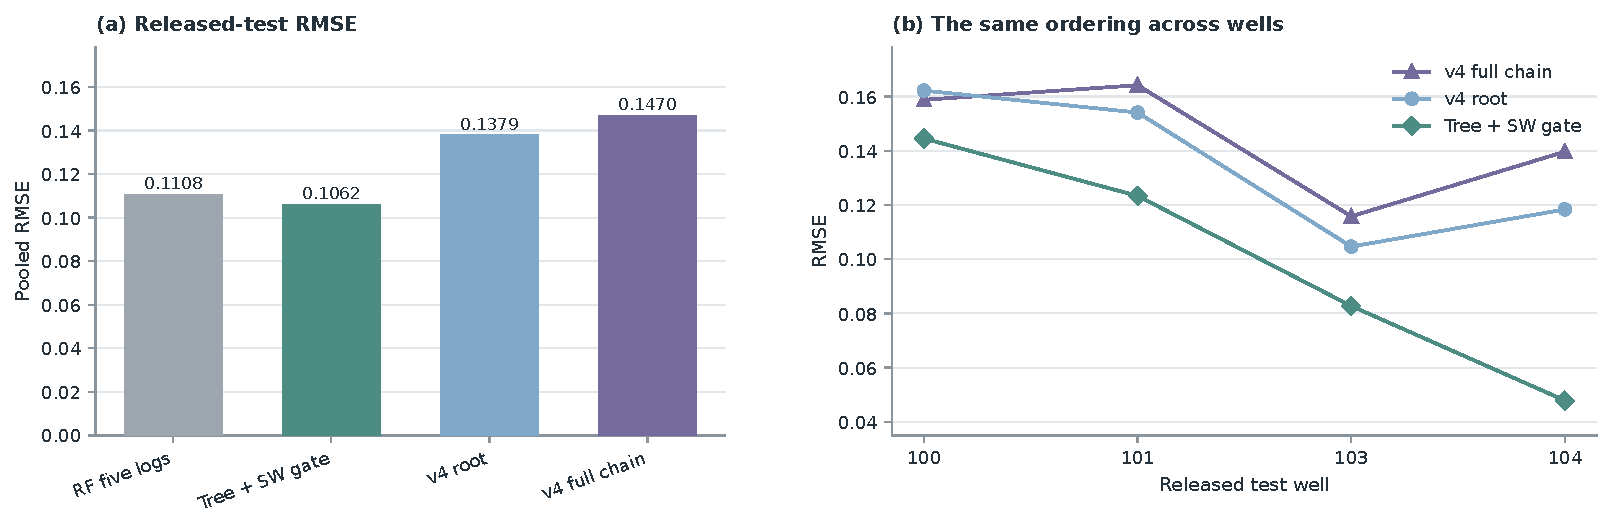
\includegraphics[width=0.88\textwidth]{figures/fig_v4_public_styled.pdf}
\caption{Public Volve transferability boundary analysis. (a) Pooled test RMSE comparing root and complete-chain v4 models against tree baselines. (b) Disaggregated per-well test RMSE across the four released boreholes, demonstrating the consistent performance advantage of tree--gate models in data-limited regimes.}
\label{fig:v4-public}
\end{figure}

\subsection{Internal complementarity and generational record}
On the internal 80-well dataset, v3 tree--sequence fusion raises the five-fold well-grouped composite score from 80.88 to 81.63. Paired well-bootstrap confidence intervals ($95\%$) for target-wise micro-score improvements strictly exclude zero: $\mathrm{POR}$ $[0.00695, 0.01282]$, $\mathrm{PERM}$ $[0.00734, 0.01082]$, and $\mathrm{SW}$ $[0.00193, 0.00655]$. At the borehole level, performance improves in 65, 72, and 47 out of the 80 individual wells for $\mathrm{POR}$, $\mathrm{PERM}$, and $\mathrm{SW}$, respectively. The lower proportion of improving wells for $\mathrm{SW}$ demonstrates that aggregate metric significance does not guarantee uniform per-well enhancement.

\begin{figure}[htbp]
\centering
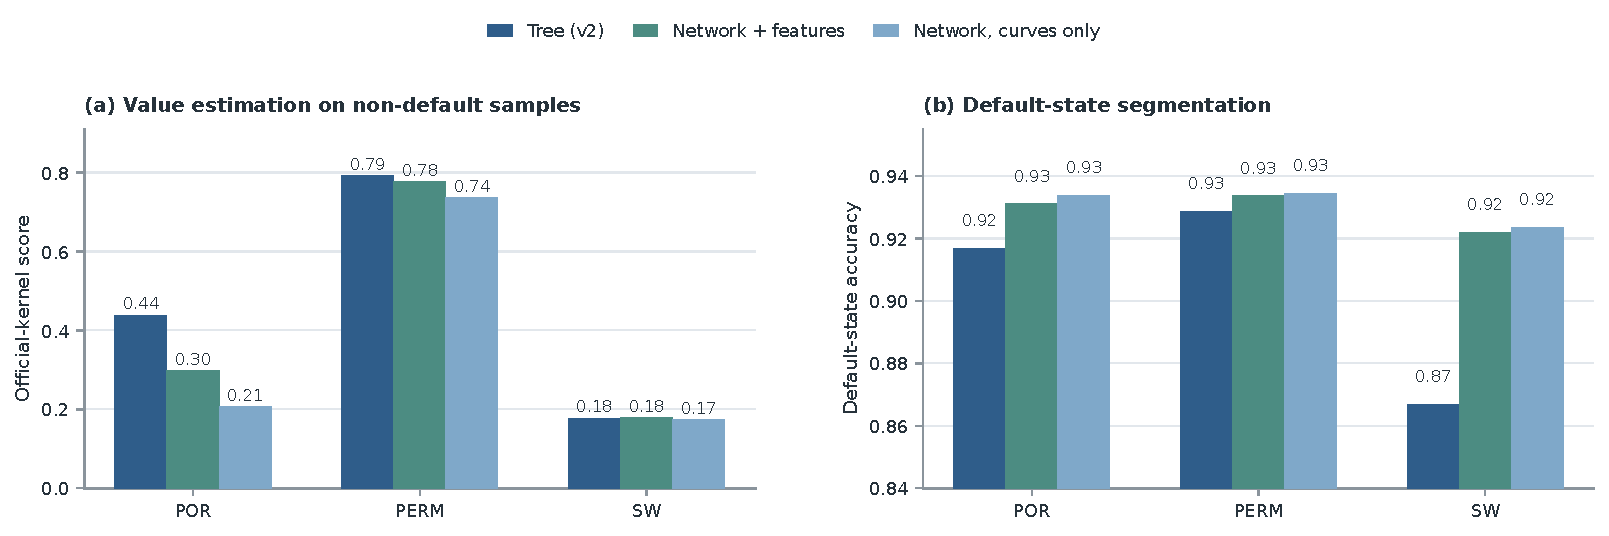
\includegraphics[width=0.75\textwidth]{figures/fig_division_clear.pdf}
\caption{Empirical division of labor between tree ensembles and deep sequence networks under identical well folds. Gradient-boosted trees provide superior local regression on non-default pay zones, whereas sequence networks excel at default-state classification, achieving the largest gain on $\mathrm{SW}$.}
\label{fig:division}
\end{figure}

Figure~\ref{fig:division} elucidates the empirical foundation of this division of labor. Under identical five-fold splits, tree models achieve higher utility on non-default reservoir intervals ($\mathrm{POR}$ utility 0.438 vs. 0.388; $\mathrm{PERM}$ utility 0.792 vs. 0.737), indicating that GBDTs are superior for continuous property mapping. In contrast, the sequence network excels at spatial boundary detection, improving default-state classification accuracy from 0.867 to 0.923 on $\mathrm{SW}$. This finding supports complementary roles under the reported protocol and motivates hierarchical distribution- and gate-level fusion. Geologically, this performance divergence correlates directly with borehole formation architecture. Point-wise tree ensembles suffer from shoulder-bed effects and instrument vertical-resolution limits across thin beds ($<0.5$\,m), abrupt lithologic transitions, and reservoir fluid boundaries, where single-depth logging readings exhibit ambiguous intermediate responses. In contrast, deep sequence networks leverage expansive vertical receptive fields to perceive surrounding stratigraphic context and depositional cyclicity, thereby resolving sharp default-state cutoffs and shaly baffle contacts with high fidelity. Conversely, within thick, homogeneous reservoir pay zones where boundary transitions are absent, tabular GBDT regression remains superior for continuous multi-sensor mapping.

\begin{table}[htbp]
\centering
\caption{Historical model-family development record on the internal industrial benchmark. Note that OOF scores are row-specific, and blind scores reflect official historical platform observations under differing development estimators.}
\label{tab:core-internal}
\resizebox{\linewidth}{!}{%
\begin{tabular}{llcc}
\toprule
Generation & Architecture description & OOF validation score & Recorded blind score \\
\midrule
v1 & Two-stage CatBoost baseline & 79.4069 & 81.0052 \\
v2 & Target-specific tree baseline & 80.8837 & 82.2718 \\
v3 & Hierarchical tree--sequence fusion & 81.6324 & 83.2579 \\
v4 & Local--global dual-backbone & 81.8910 & 83.9329 \\
v4 & Calibrated dual-backbone & 82.1744 & 83.6076 \\
v4 & Cross-family fusion & \textbf{82.2106} & 83.7159 \\
v4 & Posterior fusion & 82.1906 & 83.6394 \\
v4 & External-gate configuration & 82.1681$^*$ & \textbf{83.9377} \\
\bottomrule
\multicolumn{4}{l}{\footnotesize $^*$The external-gate configuration tunes decision thresholds on validation folds.} \\
\end{tabular}%
}
\end{table}

\newpage
Table~\ref{tab:core-internal} documents the generational progression across all developed model iterations. Cross-family fusion achieves the highest internal OOF validation score (82.2106), while the external-gate configuration records the highest historical blind observation (83.9377). Notably, ranking inversions occur across evaluation regimes: the calibrated dual-backbone gains +0.283 points in OOF cross-validation over the local--global model, but loses $-$0.325 points on the blind test wells. This divergence reinforces the principle that offline validation rankings and blind leaderboard evaluations are not interchangeable.

\subsection{Controlled fusion ablation and target heterogeneity}
The controlled full fusion configuration reproduces the original nested cross-validation score within $2.8 \times 10^{-6}$ points, confirming numerical consistency. Table~\ref{tab:controlled-ablation} reports the leave-one-module-out ablation results under strictly frozen base predictors. Removing the tabular tree distribution induces the largest performance reduction (a loss of 1.3100 composite points; $95\%$ CI $[1.1127, 1.5092]$). Sequence gates and sequence distributions contribute +0.2718 and +0.1268 points, respectively, whereas the joint-state gate provides only a marginal increment of +0.0404 points.

\begin{table}[htbp]
\centering
\caption{Controlled fusion leave-one-module-out ablation results. All experimental arms utilize identical frozen base-learner predictions, feature sets, candidate grids, and inner-fold tuning.}
\label{tab:controlled-ablation}
\resizebox{\linewidth}{!}{%
\begin{tabular}{l ccc cc}
\toprule
& \multicolumn{3}{c}{Target utility ($\bar{U}_t$)} & Composite & $\Delta$ Composite ($S$) \\
\cmidrule(lr){2-4}
Experimental arm & $\mathrm{POR}$ & $\mathrm{PERM}$ & $\mathrm{SW}$ & score ($S$) & Full $-$ ablated [95\% CI] \\
\midrule
Full fusion configuration & 0.789300 & 0.903386 & 0.752425 & 81.63236 & \textemdash \\
\quad w/o Joint-state gate & 0.789239 & 0.903015 & 0.751694 & 81.59199 & 0.0404 [0.0133, 0.0692] \\
\quad w/o Sequence gates & 0.786038 & 0.899319 & 0.751520 & 81.36053 & 0.2718 [0.2249, 0.3239] \\
\quad w/o Sequence distributions & 0.789300 & 0.902695 & 0.749493 & 81.50556 & 0.1268 [0.0588, 0.2063] \\
\quad w/o Tabular tree distribution & 0.752674 & 0.897849 & 0.751927 & 80.32240 & 1.3100 [1.1127, 1.5092] \\
\bottomrule
\end{tabular}%
}
\end{table}

Importantly, the ablation results clarify why each module appears to yield a positive contribution at the composite score level ($S$), while displaying zero or neutral benefit at the individual target level. Because the composite score is a linear weighted sum across the three properties ($S = 100(0.30\bar{U}_{\mathrm{POR}} + 0.35\bar{U}_{\mathrm{PERM}} + 0.35\bar{U}_{\mathrm{SW}})$), an architectural component that improves even a single target can produce a positive composite delta; whether its confidence interval excludes zero must be assessed separately. Disaggregating performance by target reveals that this composite gain is non-uniform across individual petrophysical properties:
\begin{itemize}
\item Removing the joint-state gate produces no statistically distinguishable effect on $\mathrm{POR}$ (delta = 0.000060; $95\%$ CI $[-0.000394, 0.000553]$, encompassing zero).
\item Sequence distributions are not selected for $\mathrm{POR}$ by inner-fold tuning, resulting in an exact delta of 0.000000.
\item The sequence distribution effect on $\mathrm{PERM}$ is negligible, with its bootstrap confidence interval spanning zero ($[-0.000005, 0.001434]$).
\end{itemize}
Furthermore, the $2 \times 2$ factorial interaction between sequence distributions and the joint-state gate is negligible (0.000000 for $\mathrm{POR}$, 0.000033 for $\mathrm{PERM}$, and 0.000345 for $\mathrm{SW}$). The composite interaction magnitude (+0.0132 points; $95\%$ CI $[0.0041, 0.0211]$), while technically resolvable via bootstrap, is practically insufficient to alter model selection. These target-decoupled findings argue against interpreting the results as uniform monotonic increments across all components; composite gains instead reflect target-selective representational complementarity.

\subsection{Hyperparameter sensitivity and ranking stability}
Figure~\ref{fig:sensitivity} details the systematic hyperparameter sweeps conducted to evaluate model stability. Across all five cross-validation folds, inner-fold grid optimization selects identical continuous tree weights ($\alpha_{\mathrm{POR}} = 1.00$, $\alpha_{\mathrm{PERM}} = 0.75$, and $\alpha_{\mathrm{SW}} = 0.50$). Concurrently, discrete decision gating thresholds exhibit minimal fold dispersion: $\tau_{\mathrm{POR}} \in [0.22, 0.27]$ (four folds at 0.27, one at 0.22), $\tau_{\mathrm{PERM}} \in [0.41, 0.44]$, and $\tau_{\mathrm{SW}}$ is identically $0.07$ across all five folds, directly confirming inner-fold selection consistency. In contrast, discrete decision threshold sensitivity varies substantially across properties under global sweeps: while $60.7\%$ and $64.0\%$ of tested thresholds maintain the full configuration above the v2 baseline for $\mathrm{POR}$ and $\mathrm{PERM}$, respectively, only $21.3\%$ of candidate thresholds preserve this advantage for $\mathrm{SW}$ (Fig.~\ref{fig:sensitivity}b). This shows that performance gains on water saturation are threshold-sensitive rather than broadly unconditional.

\begin{figure}[t]
\centering
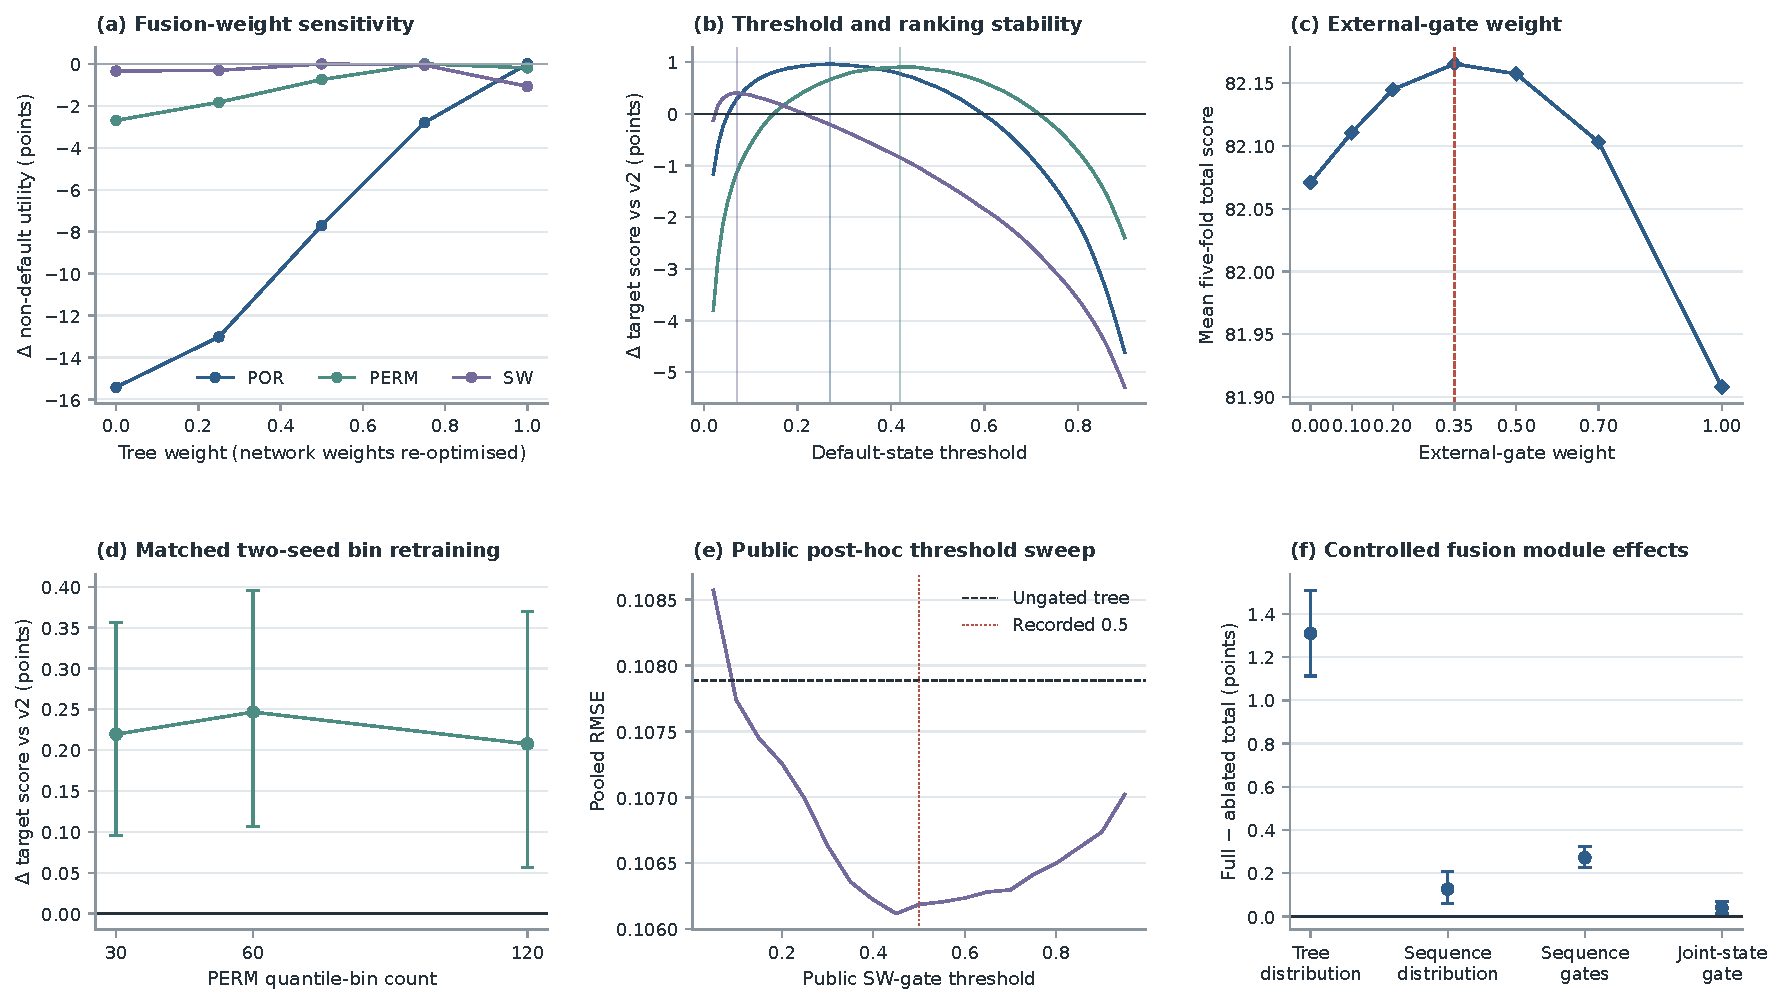
\includegraphics[width=\textwidth]{figures/reviewer_sensitivity.pdf}
\caption{Systematic hyperparameter sensitivity and ablation analysis. (a) Marginal sensitivity of continuous fusion weights. (b) Internal decision threshold sweeps relative to the v2 baseline. (c) Frozen external-gate weight sweep across folds. (d) Matched two-seed retraining across $\mathrm{PERM}$ quantile bin counts. (e) Public Volve released-test threshold sweep. (f) Leave-one-module-out ablation impacts with well-bootstrap confidence intervals.}
\label{fig:sensitivity}
\end{figure}

Sweeping the external-gate blending weight ($w_{\mathrm{ext}}$) from 0.10 to 0.50 yields improvements across all five folds relative to unblended predictions ($w_{\mathrm{ext}} = 0$). The historical setting of 0.35 attains the highest mean fold score (82.165 vs. 82.071 at weight zero), whereas an exclusively external gate degrades performance to 81.908 (Fig.~\ref{fig:sensitivity}c). The per-fold optimal weight varies between 0.20 and 0.50, demonstrating the value of moderate ensemble blending without supporting a single precise optimum across folds.

On the public Volve benchmark, 18 of the 19 evaluated $\mathrm{SW}$ decision thresholds improve pooled RMSE over the ungated tree (Fig.~\ref{fig:sensitivity}e). The post-hoc optimum occurs at $\tau = 0.45$ (RMSE 0.106118), representing an immaterial difference of only 0.000069 relative to the default 0.50 setting. This supports pooled threshold robustness while preserving the observed per-well heterogeneity.

Finally, matched retraining of permeability models across $K \in \{30, 60, 120\}$ quantile bins demonstrates non-monotonic scaling. Target scores are 0.89662, 0.89689, and 0.89650 for 30, 60, and 120 bins, respectively. Although 60 bins emerges as optimal in four out of five folds ($92.4\%$ of bootstrap resamples), the score variations across bin granularities remain within narrow, stable bounds: $30 - 60$ bins yields $-0.000271$ ($95\%$ CI $[-0.000600, 0.000098]$), while $60 - 120$ bins yields $+0.000390$ ($95\%$ CI $[0.000103, 0.000704]$). Performance does not scale monotonically with bin density, confirming that fine-grained quantization yields diminishing returns.

\section{Negative and neutral controls}
\label{sec:negative}
To comprehensively delineate the operational envelope and architectural trade-offs of the predictive framework, Table~\ref{tab:negative} catalogs the empirical negative and neutral controls identified during systematic investigation. Specifically, substituting a 60-bin continuous distribution for $\mathrm{SW}$ yields a slight utility change from 0.7484 to 0.7475 (with the paired confidence interval spanning zero), demonstrating that discrete default-state categorization accounts for the predominant performance gain. Similarly, dense action grid discretization, post-hoc Platt probability calibration, median filtering, and fixed-transition Hidden Markov Models (HMMs) \cite{rabiner1989hmm} offer no measurable advantage, as time-series smoothing tends to oversmooth sharp, genuine thin-bed pay boundaries. Dynamic time warping (DTW) curve alignment produces a negligible variation from 81.63 to 81.64. On the public Volve benchmark, gating exhibits slight sensitivity on Well 101, and the complete 18-stage deep chain underperforms the baseline across all four boreholes. These neutral and negative controls substantiate that model performance is governed by specific representational synergies rather than unchecked architectural complexity.

\begin{table}[t]
\centering
\caption{Systematic summary of negative and neutral controls documented in this study.}
\label{tab:negative}
\footnotesize
\begin{tabular}{>{\raggedright\arraybackslash}p{.28\textwidth}>{\raggedright\arraybackslash}p{.38\textwidth}>{\raggedright\arraybackslash}p{.24\textwidth}}
\toprule
Investigated technique & Empirical observation & Methodological interpretation \\
\midrule
$\mathrm{SW}$ 60-bin distribution & Utility: 0.7484 $\to$ 0.7475 & Discrete atom dominates continuous spread \\
DTW curve alignment & Score: 81.63 $\to$ 81.64 & No material gain in this setting \\
Public $\mathrm{SW}$ gate (Well 101) & RMSE: 0.12295 $\to$ 0.12334 & Inter-well geological heterogeneity \\
Complete v4 chain on Volve & RMSE: 0.14695 vs. 0.10619 (tree) & Poor transfer in this setting \\
\bottomrule
\end{tabular}
\end{table}

\section{Discussion}
\label{sec:discussion}
The core insight emerging from this study is that machine-learning architectures for well-log analysis must be explicitly tailored to the underlying petrophysical failure modes and deployment metrics. Gradient-boosted trees provide robust point regression across high-dimensional feature spaces, deep sequence networks supply vital spatial context for lithofacies boundary discrimination, and metric-aligned decoding translates probabilistic spread into optimal engineering actions. Specifically, the architectural division of labor maps directly to physical rock-column transitions: sequence-driven models excel at demarcating thin permeable laminations, fluid contacts, and sharp lithologic boundaries where vertical context resolves instrument shoulder-bed distortions, whereas tabular trees dominate continuous value estimation within stable, homogeneous reservoir lithofacies. Furthermore, our controlled ablations emphasize that these benefits are highly target-dependent: sequence distributions are not selected for POR, whereas sequence gates can still contribute to POR state decisions.

Furthermore, these findings establish firm empirical limits on model transferability. While well-grouped validation mitigates spatial leakage, it cannot replicate the complex distribution shifts encountered across different depositional basins. The performance decline of the high-capacity 18-stage sequence pipeline on the Volve benchmark shows that complex architectures may fail to generalize when trained on sparse borehole sets.

\subsection{Operational scope and methodological boundaries}
To place these findings in rigorous engineering context, the operational boundaries of this study must be clearly demarcated. The predictive framework is data-driven, incorporating rock-physics domain knowledge through engineered feature ratios, physical boundary clipping, and discrete default-state stratification, rather than forward-simulating multi-phase fluid-flow partial differential equations (PDEs) or geological depositional processes. Furthermore, this benchmark evaluates post-drilling offline petrophysical interpretation on historical wireline logs. It does not encompass online streaming inference, Logging-While-Drilling (LWD) real-time geosteering feedback, or production history-matching loops. Consequently, the empirical conclusions apply specifically to static, retrospective reservoir formation evaluation. In operational field deployment, data-driven outputs serve to accelerate and augment expert petrophysical workflows, requiring continuous data-drift monitoring, uncertainty quantification, and local calibration against physical core plugs and well-test telemetry.

\section{Conclusions}
\label{sec:conclusions}
This study presents a comprehensive evaluation of tolerance-aware reservoir property prediction from wireline logs. On public Volve data, a target-specific tree with joint $\mathrm{SW}$ gating achieves the leading pooled RMSE of 0.10619, while the complex 18-stage sequence network fails to transfer effectively (RMSE 0.14695). On the internal 80-well benchmark, hierarchical tree--sequence fusion raises the composite score to 81.63. Controlled ablations and systematic sensitivity sweeps confirm that these performance improvements are driven by complementary state-boundary gating and robust value estimation, while exposing target-level heterogeneity and threshold sensitivities.

\section*{CRediT authorship contribution statement}
\textbf{Minjie Chen}: Conceptualization, Methodology, Software, Validation, Formal analysis, Investigation, Data curation, Writing -- original draft, Writing -- review \& editing. \textbf{Jiawei Xin}: Conceptualization, Methodology, Software, Validation, Formal analysis, Investigation, Writing -- review \& editing. \textbf{Chengfeng Wu}: Investigation, Data curation, Resources, Supervision, Writing -- review \& editing.

\section*{Declaration of competing interests}
The authors declare that they have no known competing financial interests or personal relationships that could have appeared to influence the work reported in this paper.

\section*{Declaration of generative AI and AI-assisted technologies}
The authors used generative AI tools for language refinement, code inspection and manuscript formatting, reviewed and edited the resulting content, and take responsibility for the accuracy and integrity of the work.

\section*{Data availability}
Public Volve/PDDA data are available through the SPWLA PDDA SIG repository \cite{pddasig2021}, subject to the Equinor Volve licence \cite{volve2018}. Internal benchmark data can be requested from the organizers at \url{mailto:aicomp@petrochina.com.cn}, subject to approval and governance restrictions. Aggregated results, public predictions and reproduction scripts accompany the supplementary material.

\section*{Reproducibility note}
The complete code, public reproduction pipelines, sensitivity analysis suites, and experimental artifacts are openly available on GitHub at \url{https://github.com/whiteicey/welllog-reservoir-hybrid}. The public benchmark entry point is {\small\path{reproduce_public_validation.py}}, located in {\small\path{reproducibility/public_volve/}}. Sensitivity and controlled-ablation scripts, frozen configurations, environment records, and output hashes are archived under {\small\path{experiments/reviewer_response/}}.

\section*{Acknowledgments}
The authors thank the SPWLA PDDA SIG and Equinor for releasing Volve, and the Kunlun Big Model competition organizers for providing the internal benchmark.

\section*{Funding}
This research did not receive any specific grant from funding agencies in the public, commercial or not-for-profit sectors.

\bibliographystyle{elsarticle-num}
\begingroup
\small
\setlength{\bibsep}{2.5pt}
\bibliography{refs}
\endgroup
\end{document}
